\documentclass{beamer}

\usepackage[francais]{babel}
\usepackage[utf8]{inputenc}
\usepackage[T1]{fontenc}

\usetheme{Warsaw}
\title{Intelligence Artificielle : promesses et réalités}
\author{Ouail Abed - Hakenholz Guillaume - Soufyani Amine}
\date{20 mars 2018}


\begin{document}

	\begin{frame}
	\titlepage
	\end{frame}
	
	\begin{frame} % 2eme transparent TDM générale
	\frametitle{Table des matieres}
	\tableofcontents[hideallsubsections] %ou [pausesections]
	\end{frame}

	
	\begin{frame}[fragile]
	\frametitle{Intelligence Artificielle : Definition}
	\begin{itemize}
		\item Intelligence Artificielle (IA) est « l'ensemble de théories et de techniques mises en œuvre en vue de réaliser des machines capables de simuler l'intelligence ». Elle correspond donc à un ensemble 	de concepts et de technologies plus qu'à une discipline autonome constituée.
	\end{itemize}
	\end{frame}
	
	\begin{frame}[fragile]
	\frametitle{Intelligence Artificielle : Definition}
	\begin{itemize}
		\itemsep2em
		\item Souvent classée dans le groupe des sciences cognitives, elle fait appel à la neurobiologie 					computationnelle (particulièrement aux réseaux neuronaux), à la logique mathématique et à 							l'informatique. 
		
		\item Un réseau neuronal est l’association, en un graphe plus ou moins 															complexe,d’objets élémentaires, les neurones formels qui sont eux mêmes inspirées du fonctionement 		des neuronnes biologiques
	\end{itemize}
	\end{frame}
	
	
	\begin{frame}[fragile]
	\frametitle{2 Types d'IA}
	\begin{itemize}
		\itemsep0.5em
		\item IA faible  :\\
		est une intelligence artificielle non-sensible qui se concentre sur une tâche précise
		 
		 \item IA forte: \\
		est une intelligence artificielle dotée de conscience, de sensibilité et d'esprit
		\item les systèmes actuellement existants sont considérés comme des intelligences artificielles faibles
	\end{itemize}
	\end{frame}
	
	\begin{frame}[fragile]
	\frametitle{Breve Histoire de l'IA}
	\begin{itemize}
		\itemsep0.5em
		\item (1943) La naissance des ordinateurs :\\
		 Les premiers ordinateurs voient le jour. Construits avec des technologies qui précédaient les circuits intégrés (tubes à vide, relais électromécaniques), ils sont peu performants.
		 
		 \item (1950) Le test Turing : \\
		 Le mathématicien britannique Alan Turing publie son article "Computing Machinery and Intelligence" et met au point son test à l’aveugle pour déterminer qui est l’humain ou l’ordinateur.

		 \item (1950) La première machine capable d’apprendre :\\
		 Claude Shannon développe Theseus, une souris électromécanique capable d’apprendre à trouver la sortie d’un labyrinthe. Avant même l’apparition du terme "intelligence artificielle", il s’agissait de la première démonstration effective d’une machine capable d’apprendre.

	\end{itemize}
	\end{frame}
	
	\begin{frame}[fragile]
	\frametitle{Breve Histoire de l'IA(suite)}
	\begin{itemize}
		\itemsep1em
		\item (1956) Le séminaire du Dartmouth College :\\
		 Les premiers ordinateurs voient le jour. Construits avec des technologies qui précédaient les circuits intégrés (tubes à vide, relais électromécaniques), ils sont peu performants.
		 
		 \item (1958) Le « list processing » : \\
		 John McCarthy, co-organisateur du séminaire du Dartmouth College, créé le langage informatique LISP (mot forgé à partir de l’anglais "list processing") qui permet de faciliter la programmation d’IA.

		 \item (1959) Le « General Problem Solver » :\\
		 Herbert Simon et Allen Newell inventent le General Problem Solver, une stratégie de résolution de problèmes largement utilisée dans le domaine de l'intelligence artificielle.

	\end{itemize}
	\end{frame}
	
	\begin{frame}[fragile]
	\frametitle{Breve Histoire de l'IA(suite)}
	\begin{itemize}
		\itemsep1em
		\item (1965) Le programme Eliza :\\
		 Eliza est un programme informatique écrit par Joseph Weizenbaum, capable de dialoguer en anglais en incarnant le rôle d’une psychologue.

		 \item ((1974) Le système MYCIN : \\
		 MYCIN est un système expert utilisant l’IA pour identifier des bactéries causant des infections 	sévères et recommander des antibiotiques en adaptant le dosage au poids des patients.

		 \item (1996) La victoire Deep Blue :\\
		 Le champion d’échecs Garry Kasparov est battu par le superordinateur Deep Blue d’IBM. Un événement qui démontre que l’IA est plus performante que l’homme dans certains domaines précis.

	\end{itemize}
	\end{frame}
	
	\begin{frame}[fragile]
	\frametitle{Breve Histoire de l'IA(suite)}
	\begin{itemize}
		\itemsep1em
		\item (2005) Le robot Stanley :\\
		 En 2005, Stanley, un robot construit à l’université Stanford, remporte le "DARPA Grand Challenge" en conduisant de manière autonome pendant 131 miles sur une piste de désert sans avoir fait de reconnaissance préalable
		 
		 \item (2001) Le programme Watson :\\
		 Le programme d’IA Watson d’IBM surclasse les meilleurs joueurs du jeu télévisé américain de questions réponses Jeopardy !

		 \item (2017) L’AlphaGo :\\
		 En mars 2016, le programme d’IA de Google AlphaGo bat un des meilleurs joueurs mondiaux de jeu de go, puis le 27 mai 2017, il bat le champion du monde Ke Jie.

	\end{itemize}
	\end{frame}
	
	\begin{frame}[fragile]
	\frametitle{Évolution de L'intelligence  Artificielle}
	
	\centerline{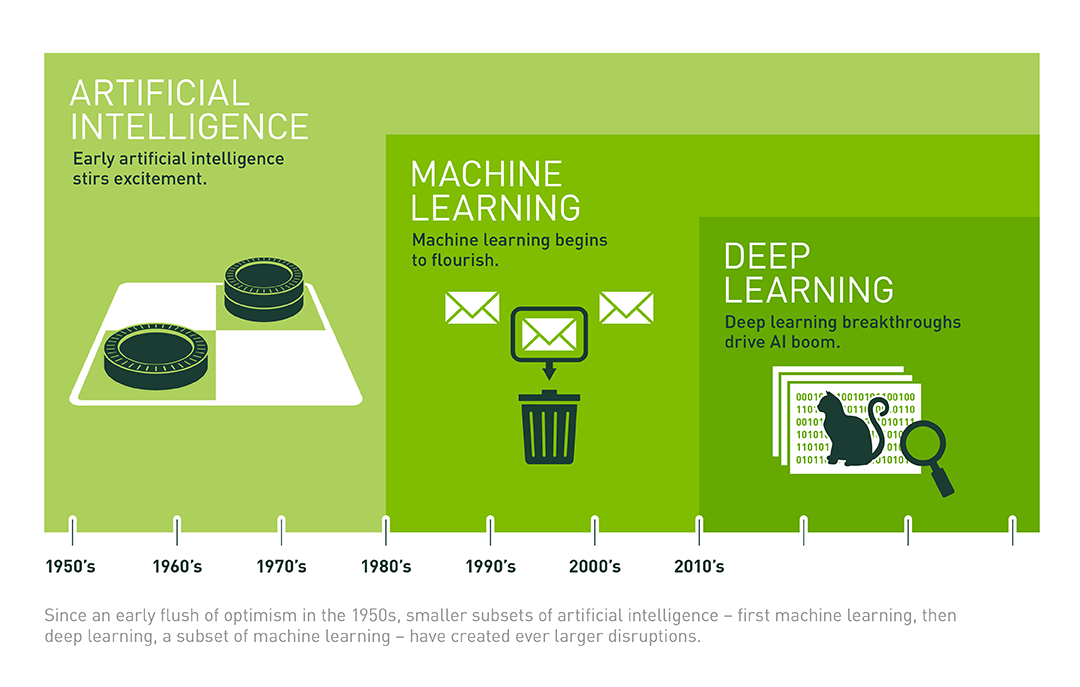
\includegraphics{evolution.png}}
	
	\end{frame}
	
	\begin{frame}[fragile]
	\frametitle{Évolution de L'intelligence  Artificielle : Machine Learning}
	\begin{itemize}
		\item Le machine learning permet à une machine d’adapter ses comportements en se fondant sur l’analyse des données à sa disposition. Un robot peut ainsi apprendre à marcher en commençant par des mouvements aléatoires, puis en sélectionnant les mouvements lui permettant d’avancer.
	\end{itemize}
	\end{frame}
	
	\begin{frame}[fragile]
	\frametitle{Évolution de L'intelligence  Artificielle : Deep Learning}
	\begin{itemize}
		\itemsep1em
		\item Le deep learning est la branche du machine learning qui utilise comme modèles mathématiques les réseaux de neurones formels, eux-mêmes construits sur la représentation mathématique et informatique d’un neurone biologique, née en 1943.
		\item  Le Deep Learning est utilisé dans la voiture autonome  de Google : le réseau de  neurones 	classifie tout l’environnement pour éviter les obstacles ou s’arrêter au bon moment 
	\end{itemize}
	\end{frame}
	
	\begin{frame}[fragile]
	\frametitle{Évolution de L'intelligence  Artificielle}
	
	\centerline{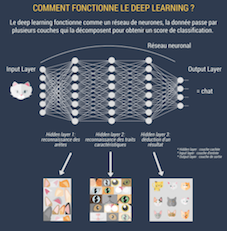
\includegraphics{deeplearning.png}}%changer pour image de meilleure qualitée
	
	\end{frame}
	
		\begin{frame}[fragile]
	\frametitle{Évolution de L'intelligence  Artificielle (fin)}
	\begin{itemize}
		\item Ces deux branches de l'intelligence artificielle ont causées de grandes améliorations de algorithmes, mais malgres cela l'IA d'aujourd'hui est est toujours qualifiée de « faible », en opposition à l’IA « forte » et consciente d’elle-même que prédisent les transhumanistes.

	\end{itemize}
	\end{frame}
	
	%%%%%%%%%%%%%%%%%%%%%%%%%
	%    Les Réalités       %
	%%%%%%%%%%%%%%%%%%%%%%%%%
	
	\begin{frame}[fragile]
	\frametitle{Les Réalités de l'Intelligence Artificielle}
	\begin{block}{Les utilisations de l'IA}
	\begin{itemize}
	\itemsep1em
		\item On peut imaginer plein de possibilité avec l'IA que se soit :
		\begin{itemize}
		\itemsep1em
		\item L'automobile
		\item L'industriel
		\item L'armée
		\item Le médical
		\item Le jeu-vidéo
		\item La téléphonie
		\item ...
		\end{itemize}
		\end{itemize}
	\end{block}
	\end{frame}
	
	\begin{frame}[fragile]
	\frametitle{Les Réalités de l'Intelligence Artificielle}
	\begin{block}{Les utilisations de l'IA}
	\begin{itemize}
	\itemsep1em
		\item De nos jours il existe plein de projets en développement et en prototype :
		\begin{itemize}
		\itemsep1em
		\item Le SolarXOne est un drone autonome mis au point par la société Xsun et la collaboration de l’école Centrale Nantes, Dassault systèmes mais aussi Airbus. Il se recharge à l'énergie solaire et l'IA intégrée lui permet de décider, seul, de sa trajectoire en fonction de la destination mais aussi de faire attention à de différents facteurs tels que la météo.
		\item La Renault Symbioz est une voiture autonome. Elle possède 35 capteurs tout au tour d'elle. L'IA permet de conduire automatiquement sur autoroute, et passer des péages
		\item Le Robot Sophia est un robot qui possède des expressions faciales en fonction du contexte, peut répondre à des questions et enregistre les différents visages de ses interlocuteurs
		\end{itemize}
		\end{itemize}
	\end{block}
	\end{frame}
	
	\begin{frame}[fragile]
	\frametitle{Les Réalités de l'Intelligence Artificielle}
	\begin{block}{Les utilisations de l'IA}
	\begin{itemize}
	\itemsep1em
		\item Dans l'industriel, les tâches répétitives ne sont plus effectuées par des humains mais par des machines programmées, ce concept est généralement adopté par les usines automobiles.
		\item Dans le médical, il existe des systèmes experts qui sont utilisés pour aider à diagnostiquer des patients.
		\item Dans le jeu-vidéo, avec l'ordinateur qui doit essayer de jouer aussi bien que l'humain pour même essayer de le battre suivant la difficulté choisie par le joueur.
		\item Dans la téléphonie, les Smartphones incorporent une multitude de programmes d'intelligence artificielle comme la reconnaissance vocale, la reconnaissance faciale ect ...
	\end{itemize}
	\end{block}
	\end{frame}
	
	%%%%%%%%%%%%%%%%%%%%%%%%%
	%     Les Dangers       %
	%%%%%%%%%%%%%%%%%%%%%%%%%
	
	\begin{frame}[fragile]
	\frametitle{Les Dangers de l'Intelligence Artificielle}
	\begin{block}{Les inquiétudes sur l'IA}
	\begin{itemize}
	\itemsep1em
		\item En 2014, Stephen Hawking met en garde sur le risque que l'IA devienne plus intelligente que l'Homme et le domine
		\item Moshe Vardi, un spécialiste américain de l'informatique, suppose que l'IA pourrait mettre 50\% de l'humanité au chômage
		\end{itemize}
	\end{block}

	\end{frame}
	
	\begin{frame}[fragile]
	\frametitle{Les Dangers de l'Intelligence Artificielle}
	\begin{itemize}
	\itemsep1em
		\item En Février 2018, 26 experts spécialistes en intelligence artificielle mettent en garde contre les dangers d'un usage criminelle de l'IA : augmentation de la la cybercriminalité , conduire à des utilisations de drones ou de robots à des fins terroristes, etc...
		\item Selon eux, dans les dix prochaines années, l'efficacité croissante de l'IA risque de renforcer la cybercriminalité mais aussi de conduire à des utilisations de drones ou de robots à des fins terroristes
		\item Moshe Vardi, un spécialiste américain de l'informatique, suppose que l'IA pourrait mettre 50\% de l'humanité au chômage
		\end{itemize}
	\end{frame}

	\begin{frame}[fragile]
	\frametitle{Les Dangers de l'Intelligence Artificielle}
	\framesubtitle{Google Home}
	\centerline{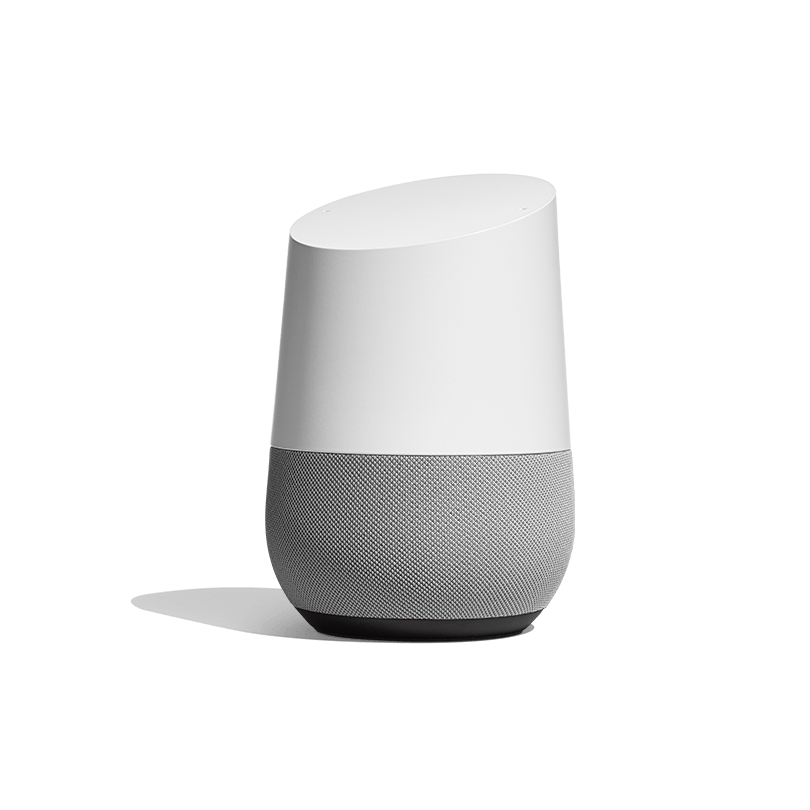
\includegraphics[height=8cm]{googlehome.png}}
	\end{frame}
	
	\begin{frame}[fragile]
	\frametitle{Les Dangers de l'Intelligence Artificielle}
	\framesubtitle{Google Home}
	\begin{block}{Google Home}
	\begin{itemize}
	\itemsep1em
		\item Le Google Assistant est une IA inclus dans le Google Home
		\item On peut lui poser toutes sortes de questions ou lui demander des services (Planifier votre journée, Contrôler votre maison connectée, Gérer les tâches...)
		\item Toutes actions sur le Google Home est enregistré et peut-être détourné de façon commerciale ou malveillante
	\end{itemize}
	\end{block}
	\end{frame}
	
	\begin{frame}[fragile]
	\frametitle{Les Dangers de l'Intelligence Artificielle}
	\framesubtitle{Drones Autonomes}
	\centerline{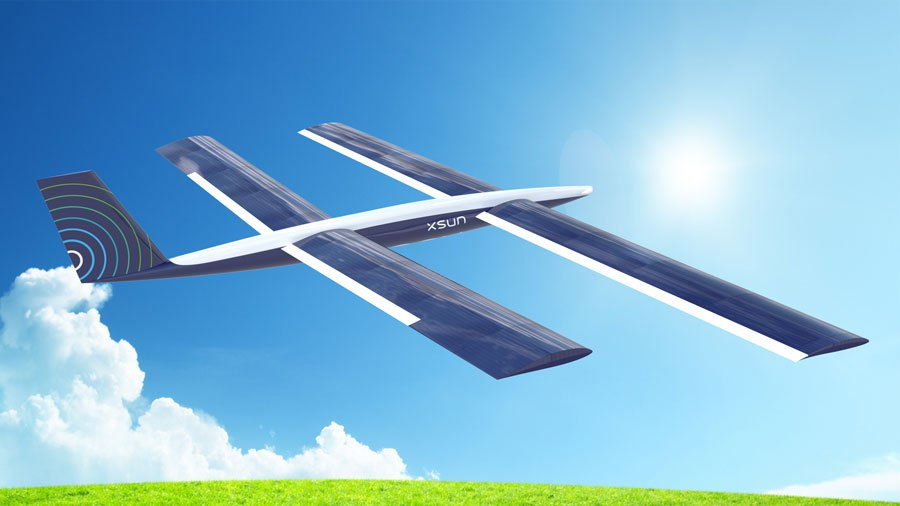
\includegraphics[height=6cm]{drone.jpg}}
	\end{frame}
	
	\begin{frame}[fragile]
	\frametitle{Les Dangers de l'Intelligence Artificielle}
	\framesubtitle{Drones Autonomes}
	\begin{block}{Drones Autonomes}
	\begin{itemize}
	\itemsep1em
		\item La Nasa dévoloppe des Drones Autonomes utilisant la technologie de Google nommé Tango qui permet de faire une cartographie 3D en temps réel
		\item Pour la Nasa, et Google, le principal intérêt de cette expérimentation est d'utiliser la Technologie Tango en alternative au GPS pour évoluer à l'intérieur des bâtiments. Cette technologie pourrait se retrouver un jour sur des drones ou des robots amenés à travailler dans des entrepôts ou à évoluer sur des zones sinistrées lors de missions de sauvetage
		\item Des Drones Autonomes pourraient servir d'armes pour l'Armée. La CCAC (Convention sur certaines armes classiques) n'ont pas abouti à des décisions concrètes sur l'utilisation des Drones Autonomes
	\end{itemize}
	\end{block}
	\end{frame}
	
	\begin{frame}[fragile]
	\frametitle{Les Dangers de l'Intelligence Artificielle}
	\framesubtitle{Voitures Autonomes}
	\centerline{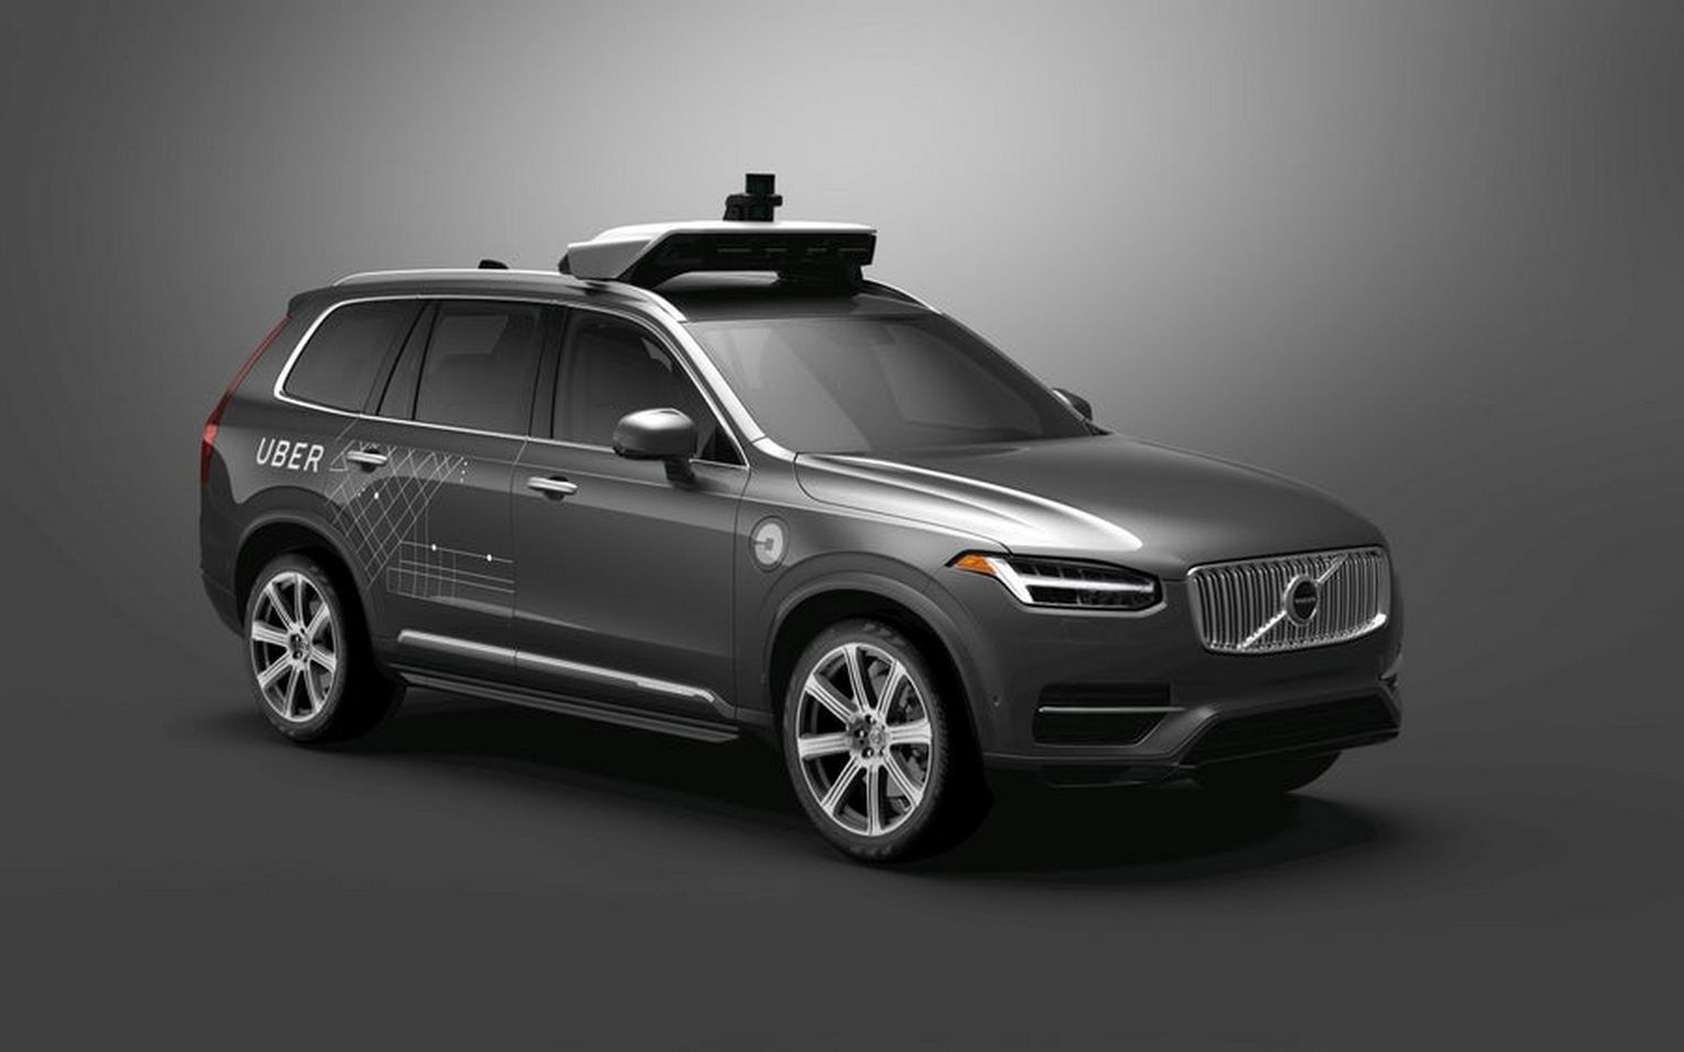
\includegraphics[height=6cm]{uber.jpg}}
	\end{frame}
	
	\begin{frame}[fragile]
	\frametitle{Les Dangers de l'Intelligence Artificielle}
	\framesubtitle{Voitures Autonomes}
	\begin{block}{Voitures Autonomes}
	\begin{itemize}
	\itemsep1em
		\item Les voitures autonomes sont conçus pour être conduite par une IA
		\item La sécurité est le point le plus important et ce n'est pas toujours parfait
		\item Le 19 Mars 2018, un accident mortel entre une voiture autonome et un piéton
		\item Le MIT (Massachusetts Institute of Technology) ont développé un test nommé Moral Machine pour tester les humains sur des questions morales
	\end{itemize}
	\end{block}
	\end{frame}
	
	\begin{frame}[fragile]
	\frametitle{Les Dangers de l'Intelligence Artificielle}
	\framesubtitle{Voitures Autonomes}
	\centerline{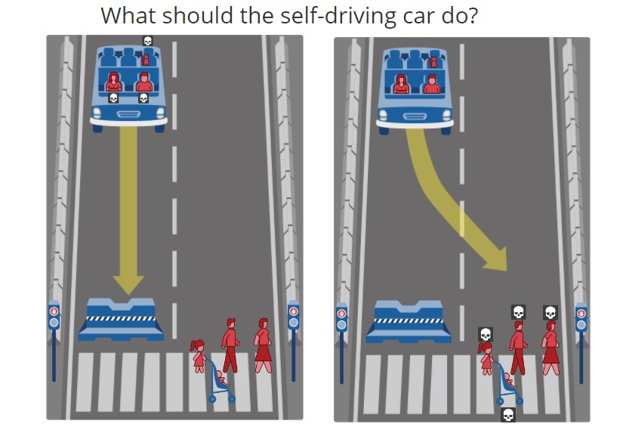
\includegraphics[height=6cm]{MIT.jpg}}
	\end{frame}
	
	\begin{frame}[fragile]
	\frametitle{Les Dangers de l'Intelligence Artificielle}
	\framesubtitle{Voitures Autonomes}
	\centerline{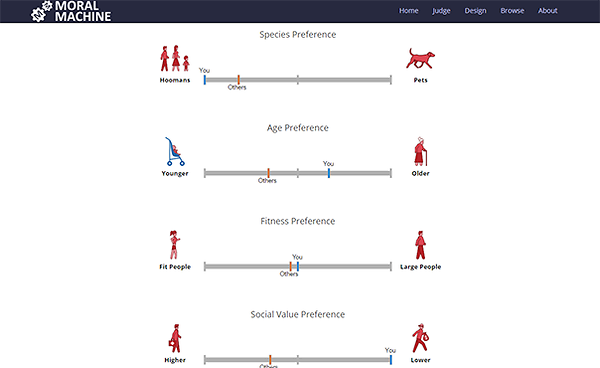
\includegraphics[height=6cm]{MIT2.png}}
	\end{frame}
	
	\begin{frame}[fragile]
	\frametitle{Les Dangers de l'Intelligence Artificielle}
	\framesubtitle{Robots, Humanoïdes}
	\centerline{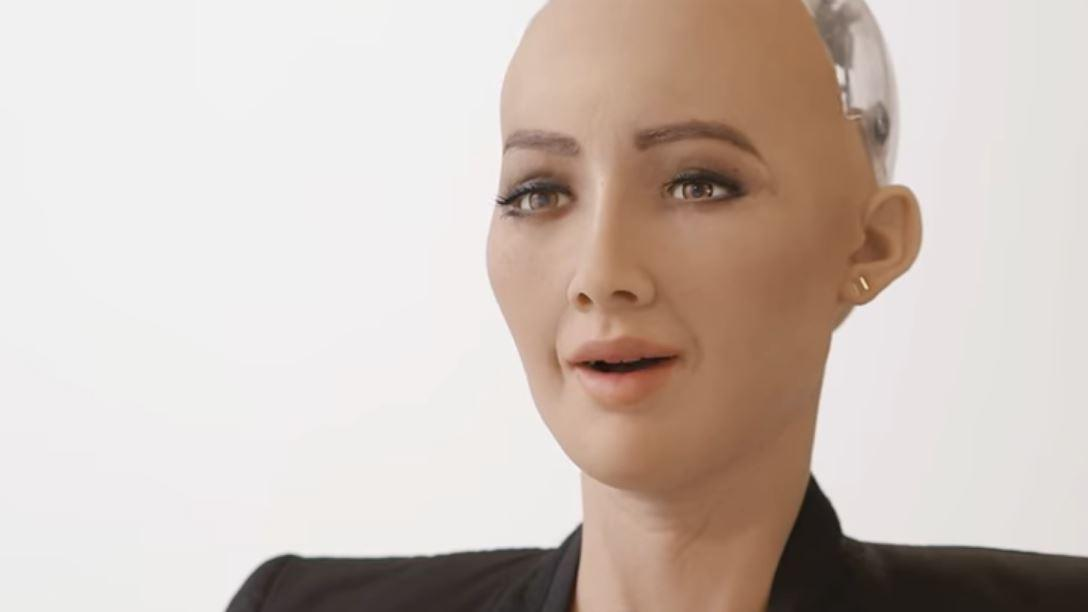
\includegraphics[height=6cm]{robotSophia.jpeg}}
	\end{frame}
	
	\begin{frame}[fragile]
	\frametitle{Les Dangers de l'Intelligence Artificielle}
	\framesubtitle{Robots, Humanoïdes}
	\centerline{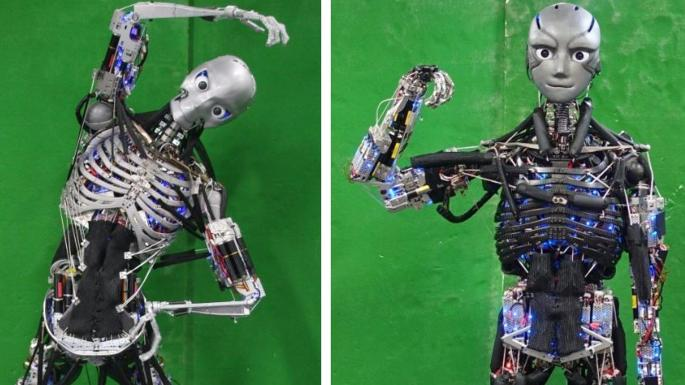
\includegraphics[height=6cm]{kenshiro_kengoro.jpg}}
	\end{frame}
	
		\begin{frame}[fragile]
	\frametitle{Les Dangers de l'Intelligence Artificielle}
	\framesubtitle{Robots, Humanoïdes}
	\begin{block}{Robots, Humanoïdes}
	\begin{itemize}
	\itemsep1em
		\item Isaac Asimov a créé les 3 lois de la Robotique :
		\begin{itemize}
		\itemsep1em
			\item Première loi : Un robot ne peut porter atteinte à un être humain ni, restant passif, laisser cet être humain exposé au danger.
			\item Deuxième loi : Un robot doit obéir aux ordres donnés par les êtres humains, sauf si de tels ordres sont en contradiction avec la première loi.
			\item Troisième loi : Un robot doit protéger son existence dans la mesure ou cette protection n'est pas en contradiction avec la première ou la deuxième loi.
		\end{itemize}
		\item Beaucoup de films traitent le sujet des dangers avec les Humanoïdes
	\end{itemize}
	\end{block}
	\end{frame}
	
	\begin{frame}[fragile]
	\frametitle{Annexes}
	\begin{itemize}
	\itemsep1em
		\item Les Réalités :
		\begin{itemize}
		\itemsep1em
			\item https://www.lesnumeriques.com/voiture/renault-symbioz-demo-voiture-autonome-niveau-4-est-realite-a3433.html
			\item https://www.sciencesetavenir.fr/high-tech/intelligence-artificielle/sophia-le-robot-de-hanson-robotics-qui-va-vous-faire-peur\_103728
			\item http://tpeai.e-monsite.com/pages/i-l-etat-de-l-intelligence-artificielle-aujourd-hui.html
		\end{itemize}
		\end{itemize}
	\end{frame}	
		
	\begin{frame}[fragile]
	\frametitle{Annexes}
	\begin{itemize}
	\itemsep1em
		\item Les Dangers
		\begin{itemize}
		\itemsep1em
			\item https://fr.wikipedia.org/wiki/Intelligence\_artificielle
			\item https://www.cnas.org/publications/reports/malicious-ai-report
			\item https://www.lesechos.fr/tech-medias/hightech/0301328931624-intelligence-artificielle-un-rapport-pointe-les-risques-dune-utilisation-criminelle-2155398.php
			\item https://www.sciencesetavenir.fr/high-tech/transports/accident-mortel-entre-un-pieton-et-une-voiture-autonome-uber-la-police-publie-la-video\_122190
			\item https://www.lesechos.fr/industrie-services/automobile/0301463184693-conducteur-contre-pieton-les-dilemmes-vertigineux-de-la-voiture-autonome-2163847.php
%			\item https://start.lesechos.fr/actu-entreprises/industries/voiture-autonome-le-test-ethique-du-mit-pour-decider-qui-sauver-5897.php
			\item https://en.wikipedia.org/wiki/Moral\_Machine
			\item http://www.phonandroid.com/google-home-amazon-echo-cnil-alerte-utilisateurs-dangers-lies-a-vie-privee.html
			\item http://www.frandroid.com/produits-android/accessoires-objets-connectes/454464\_a-quoi-sert-le-google-home-lenceinte-intelligente-et-assistant-pour-la-maison
			\item https://www.futura-sciences.com/tech/actualites/drone-course-drones-ia-nasa-mesure-pilote-humain-69368/
			\item https://fr.wikipedia.org/wiki/Convention\_sur\_certaines\_armes\_classiques\#\%C3\%89volutions\_r\%C3\%A9centes
			\item https://siecledigital.fr/2016/06/10/google-tango-lenovo/
			\item https://www.sciencesetavenir.fr/high-tech/robot/ia-et-robot-citoyen-en-arabie-saoudite-un-bluff-dangereux-selon-laurence-devillers\_117933
			\item https://www.lexpress.fr/actualite/sciences/video-kengoro-le-robot-ultra-perfectionne-qui-transpire-quand-il-fait-des-pompes\_1972852.html
		\end{itemize}
		\end{itemize}
	\end{frame}
	
	\begin{frame}[fragile]
	\frametitle{Annexes}
	\begin{itemize}
	\itemsep1em
		\item https://start.lesechos.fr/actu-entreprises/industries/voiture-autonome-le-test-ethique-du-mit-pour-decider-qui-sauver-5897.php
		\item https://en.wikipedia.org/wiki/Moral\_Machine
		\item http://www.phonandroid.com/google-home-amazon-echo-cnil-alerte-utilisateurs-dangers-lies-a-vie-privee.html
		\item http://www.frandroid.com/produits-android/accessoires-objets-connectes/454464\_a-quoi-sert-le-google-home-lenceinte-intelligente-et-assistant-pour-la-maison
		\item https://www.futura-sciences.com/tech/actualites/drone-course-drones-ia-nasa-mesure-pilote-humain-69368/
	\end{itemize}
	\end{frame}
	
		\begin{frame}[fragile]
	\frametitle{Annexes}
	\begin{itemize}
	\itemsep1em
		\item https://fr.wikipedia.org/wiki/Convention\_sur\_certaines\_armes\\
		\_classiques\#\%C3\%89volutions\_r\%C3\%A9centes
		\item https://siecledigital.fr/2016/06/10/google-tango-lenovo/
		\item https://www.sciencesetavenir.fr/high-tech/robot/ia-et-robot-citoyen-en-arabie-saoudite-un-bluff-dangereux-selon-laurence-devillers\_117933
		\item https://www.lexpress.fr/actualite/sciences/video-kengoro-le-robot-ultra-perfectionne-qui-transpire-quand-il-fait-des-pompes\_1972852.html
	\end{itemize}
	\end{frame}
	
\end{document}